\RestyleAlgo{boxed}
\chapter{树状层次概率计算模型}
在本章中,我们考虑将预测端词表概率进行分步求解,来解决语言模型中遇到的大词表问题。我们将这个预测端的词表用二叉树的分层的形式表示,通过多次的逻辑分类算法判断二叉树的访问路径从而避免了对所有单词做归一化运算。为了使单词基于二叉树的路径的编码适配基于树的分层概率计算,我们首先提出了一个在二叉树分层结构上对单词进行极性编码的方案。与此同时,因为考虑到GPGPU设备上允许算法能并行计算,传统的基于CPU设备只能线性计算,这为我们算法的效率进一步提高提供了可能。为了保证算法的并行计算的高吞吐量,我们进而推导出二叉树概率模型的紧凑的代价函数以及其模型参数的梯度计算公式,使得该分层模型在GPGPU设备上的能并行地计算模型的每一层内部概率函数,而不是从根节点到叶子节点线性计地算模型内部各层的概率函数,避免浪费GPU设备的高并行性能的特性。

同时,我们需要注意到,由于所有单词都分布在这个二叉树的叶子节点上,单词的内部节点对于目前的模型无法包含单词只能作为单词的路径参数,所以需要我们在模型训练之前给一个初始化定义。然而不同算法所生成的基于二叉树上的单词分布,可能生成一颗平衡二叉树,也可能生成一颗霍夫曼二叉树,又或者是高度偏斜的二叉树,不同的树分布对其最终任务性能有很大的影响,所以应该在训练阶段之前就给出一个较为合理的单词分布。在本实验中,我们并不打算考虑那些在模型训练过程中动态交换二叉子树的算法进而调整和改变了单词在二叉子树上的分布结构, 而是采用了几种分层聚类策略,利用单词或者文本的统计信息,句法结构和语义知识和已有的层级聚类算法来初始化单词的二叉树分布结构,以达到一个稳定和可以预期的模型性能。另外,我们不考虑单词的一词多义的现象,即一个单词不会出现在两条不同的路径上,不同的的二叉树访问路径所对应的单词一定不相同。

另外,在语言模型的测试推理过程中,主要的两个任务可以分解为:1)给句子打分(Sentence Scoring)。输出给定单词序列的概率值;2)给定上下文,对所有的单词进行排序(Word Ranking)。在给定的上下文中选择获取得分最高的一个或多个候选单词。不同于传统的softmax算法情况,得到最好的候选者单词是天然可行的并且能直接被计算出来,层次推理模型不能直接应用 softmax 方法来实现。尽管我们可以计算出所有单词的概率,然后再依照softmax算法的情况类推,这样的计算方式是十分冗余的,直接将层次模型的计算优点给忽略了。因此,我们需要讨论并研究基于二叉树的搜索策略,以满足上述两种不同的推理情形。
\section{基于二叉树的单词极性编码}
首先,我们需要知道所有的单词分布在二叉树的叶节点上,因此我们可以通过访问从根到叶节点的所有内部节点来定位每个特定的词,所以不同的访问路径代表不同的单词。举例来说,单词~$w$~的路径表示所有内部节点~$\theta^w_i$~和它访问的边~$d^w_i$。

为了方便理解,首先直观上说明一下传统softmax和树状层次概率模型的差异点。可以认为传统的softmax将单词均匀放置在一个特征空间(Feature Space)里面。基于二叉树的算法则是首先将这个所有单词所在的特征空间划分成两个子空间(Subspace),这里需要注意的是,我们没有规定空间划分必须均匀(Equal Partition),所以这两个子空间不一定相同。接下来,对每一个子空间,接着划分成两个更小的子空间,直到每个子空间里面包含的单词有且仅有一个为止。在模型计算概率的时候,更多的时候是计算特征划分到这个子空间的概率。
因此每次都需要计算二叉树访问路径的概率,这个概率值就是将模拟特征划分到这个子空间的可能性。
通过这个路径概率的求和我们可以避免对所有单词的概率计算,因为每次都做逻辑分类算法(Logistic Classification),只要计算一个分支的概率,由于两个分支的概率值之和一定等于1,另一个分支的概率可以直接推导出来,从而不需要再计算一遍了。


接下来,来说明传统二叉树编码和我们提出的编码方案之间的差异点。不同于传统的基于二叉树的单词的~$0,1$~编码方案,在模型中需要引入单词的极性编码方案(Polarity Encoding Scheme),即单词的路径是由$-1,+1$组成。其含义同原来的01编码方案类似,但他能帮助推导出更加简洁有效的模型代价函数。在上一章中,图~\ref{fig:case_thsm}~给展示了一个路径编码的例子。

\begin{table}[!t]
  \centering
  \caption{树状层次概率计算模型的符号助记表\label{tab:note}}
\begin{tabular}{llc}
  \toprule
   符号&含义&取值范围\\ \midrule
$l^w$ &单词$w$ 所对应的叶子节点和中间节点的路径&Int32 \\
$d_j$&表示路径$l^w$中第$j$个节点对应的编码(根节点对应编码$0$)&$ \{-1,+1\}$\\
$ d^w=[d_0^w,d_1^w,\cdots,d_{l^w-1}^w] $& 单词 $w$ 的极性编码,他由 $l^w-1$位编码构成,&$\{-1,+1\}^{l_w}$\\
$\theta_{j}^w\in\mathbb{R}^m$ &表示路径$l^w$中第 $j$ 个非叶子节点对应的向量& Float32\\
$ \theta^w=[\theta_1^w,\theta_2^w,\theta_3^w, \cdots,\theta_{l^w}^w]$&表示路径$l^w$所对应的参数矩阵&Float32 \\
$\Gamma$ &路径查找表,给定路径序列,可以获得对应的单词& ---\\
  \bottomrule
\end{tabular}
\end{table}

由于实际层次聚类算法(Hierarchical Agglomerative Clustering)产生的二叉树分布通常是不平衡的,所以不同单词的路径长度不一致,然而基于python语言的Numpy和Theano库目前都不支持动态长度的设置(Dynamic Type),所以需要介绍一下实际实现过程中用到的辅助计算矩阵,其结果和使用C++等动态语言所计算输出的结果是一致的,仅仅是因为实现语言框架的限制,导致引入这一操作。
需要注意到,对于平衡二叉树,所有单词的访问路径长度是一样的,所以不需要使用掩码矩阵。
对于非平衡二叉树,由于单词的访问路径长度都不是很相似,因此我们可以使用掩码矩阵来进行计算,在这里掩码矩阵标记为$\mathtt{bitmask}$。
当使用掩码矩阵时,相当于将非平衡二叉树填补形成一颗完全二叉树,如图~\ref{fig:case_thsm_mask}~所示。但是那些填补单词的子树都代表该单词,即:存在多条路径指代同一个单词,而在实际求解实验过程中,需要保证一条路径只对应一个单词,因为多余的计算路径会被掩码覆盖掉,无法反映在实际模型的代价函数里面。


接下来详细说明模型的编码方式和所涉及的参数,如表~\ref{tab:note}~所示。其中,$\theta_i^w $表示到达叶子单词节点$w$的路径上第~$i^{th}$~层上的非叶节点,并且$\theta_i ^ w$是一个 $m$维度的向量,即:$\theta_i^w \in\mathbb{R}^m $ 其中$ i \in [0, l^w-1] $。同样的,$ d_i^w $表示连接第$(i-1)^{th}$层和第$i^{th}$层节点的边。对于每个非叶子节点来说,向下移动到左边的分支标记为$ -1 $,选择右边的分支标记为$ + 1 $。因此:$i\in[0,l^w-1]$, $d_i^w\in \{-1,+1\}$。 除此之外, $l^w$~表示从根节点到叶子单词节点的路径长度。如果该二叉树是平衡树,即单词都均匀分布在同一层叶子节点上,那么二叉树的深度(Tree Depth)是$l^w\approx \log \mathcal{|V|}$ 。通过这个编码方案,可以使用极性路径来定位每个单词,即:将单词索引(Indexing)或稀疏向量表示(Sparse Representation)改变为单词极性编码元组$(d^w,\theta^w)$。



在实际运行环境中,需要通过维护一个路径查找表$\Gamma$(Path Looking-up Table),用来记住每个单词$ w $从根到叶的所有访问内部节点的索引。这样,就可以从$ \Gamma(w)$中选择对应行的所有节点,从参数矩阵${\Theta} $中检索$ \theta ^ w $。其中${\Theta} $的第一维的维度是:
\begin{equation}\label{equ:sums}
\sum_{i=0}^{\log \mathcal{|V|}}{2^i} =2^0+2^1+\cdots+2^{\log \mathcal{|V|}}= \mathcal{|V|} -1.
\end{equation}
因此,p-tHSM模型没有增加模型额外参数,除了预先给定的路径查找表$\Gamma$和预先定义的路径掩码矩阵$\mathtt{bitmask}$。


\begin{figure}[!t]
  \centering
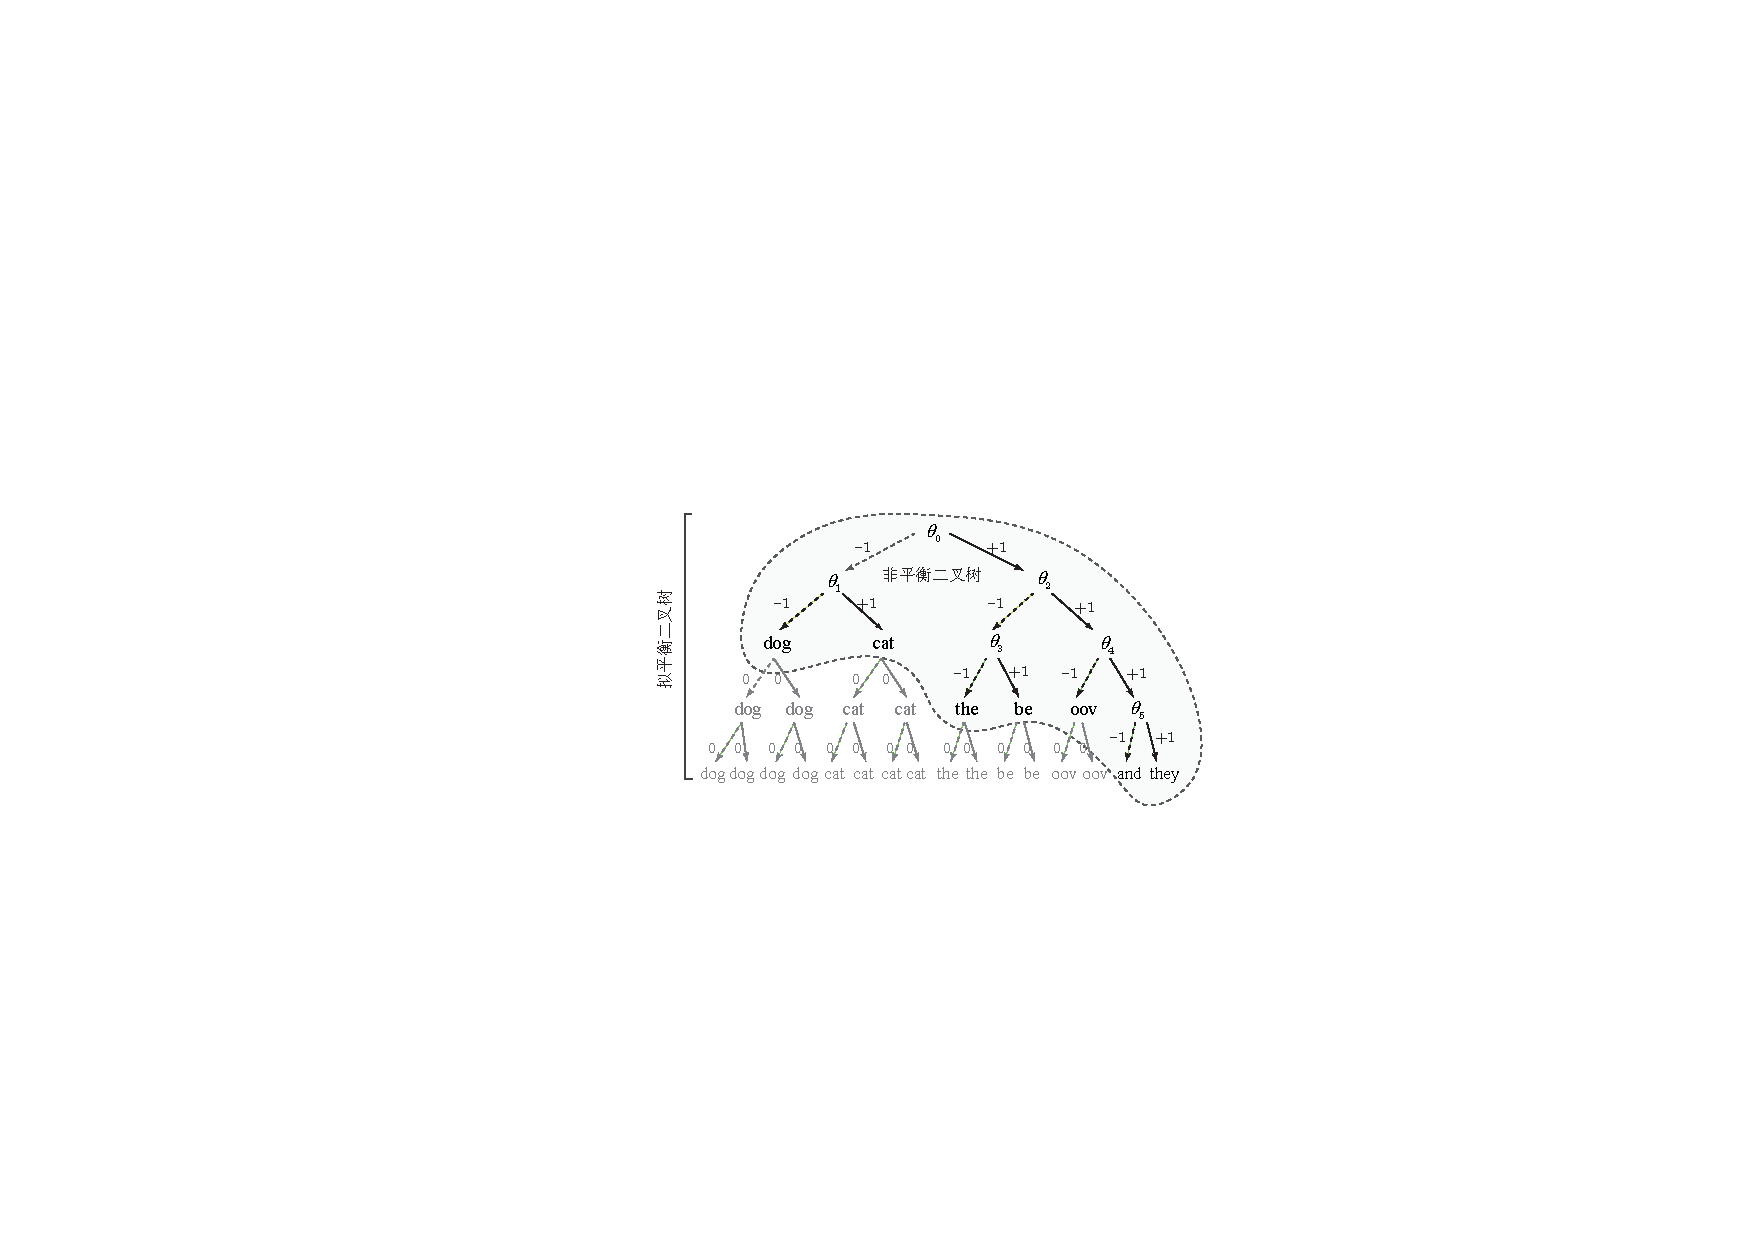
\includegraphics[width=0.85\linewidth]{./figures/thsm-example-mask.pdf}
\caption{非平衡二叉树调整成平衡二叉树}\label{fig:case_thsm_mask}
\end{figure}




除此以外,需要从矩阵$\mathcal{D}$中获得第~$w^{th}$~行向量来检索$d^w$,这里所指的$w$是词汇表中的单词索引而不是字符单词,即:$w\in [0,\mathcal{|V|}-1]$。 此外,我们需要区分模型的不同参数是在不同阶段确定的:$\{\Gamma,\mathcal{D}\}$ 是由层次聚类算法预先给定的,$\Theta$是通过训练数据集上的代价函数的梯度下降来优化的。模型实际调用的各个参数取值如表~\ref{tab:example}~所示。

\begin{table}[!h]
  \centering
  \caption{p-tHSM算法的编码和参数样例结果}\label{tab:example}
\begin{tabular}{lll}
  \toprule
  词表&路径查找表$\Gamma$& 单词路径参数\\ \midrule
dog & -1,-1,0,0,0& $\theta_0,\theta_1$\\
cat & -1,+1,0,0,0&$\theta_0,\theta_1$\\
the & -1,-1,0,0,0& $\theta_0,\theta_2,\theta_3$\\
be & -1,+1,0,0,0&$\theta_0,\theta_2,\theta_3$\\
oov & -1,+1,0,0,0&$\theta_0,\theta_2,\theta_4$\\
and & +1,+1,+1,-1& $\theta_0,\theta_2,\theta_5$\\
they & +1,+1,+1,+1&$\theta_0,\theta_1,\theta_5$\\
  \bottomrule
\end{tabular}
\end{table}

\begin{figure}[!h]
  \centering
    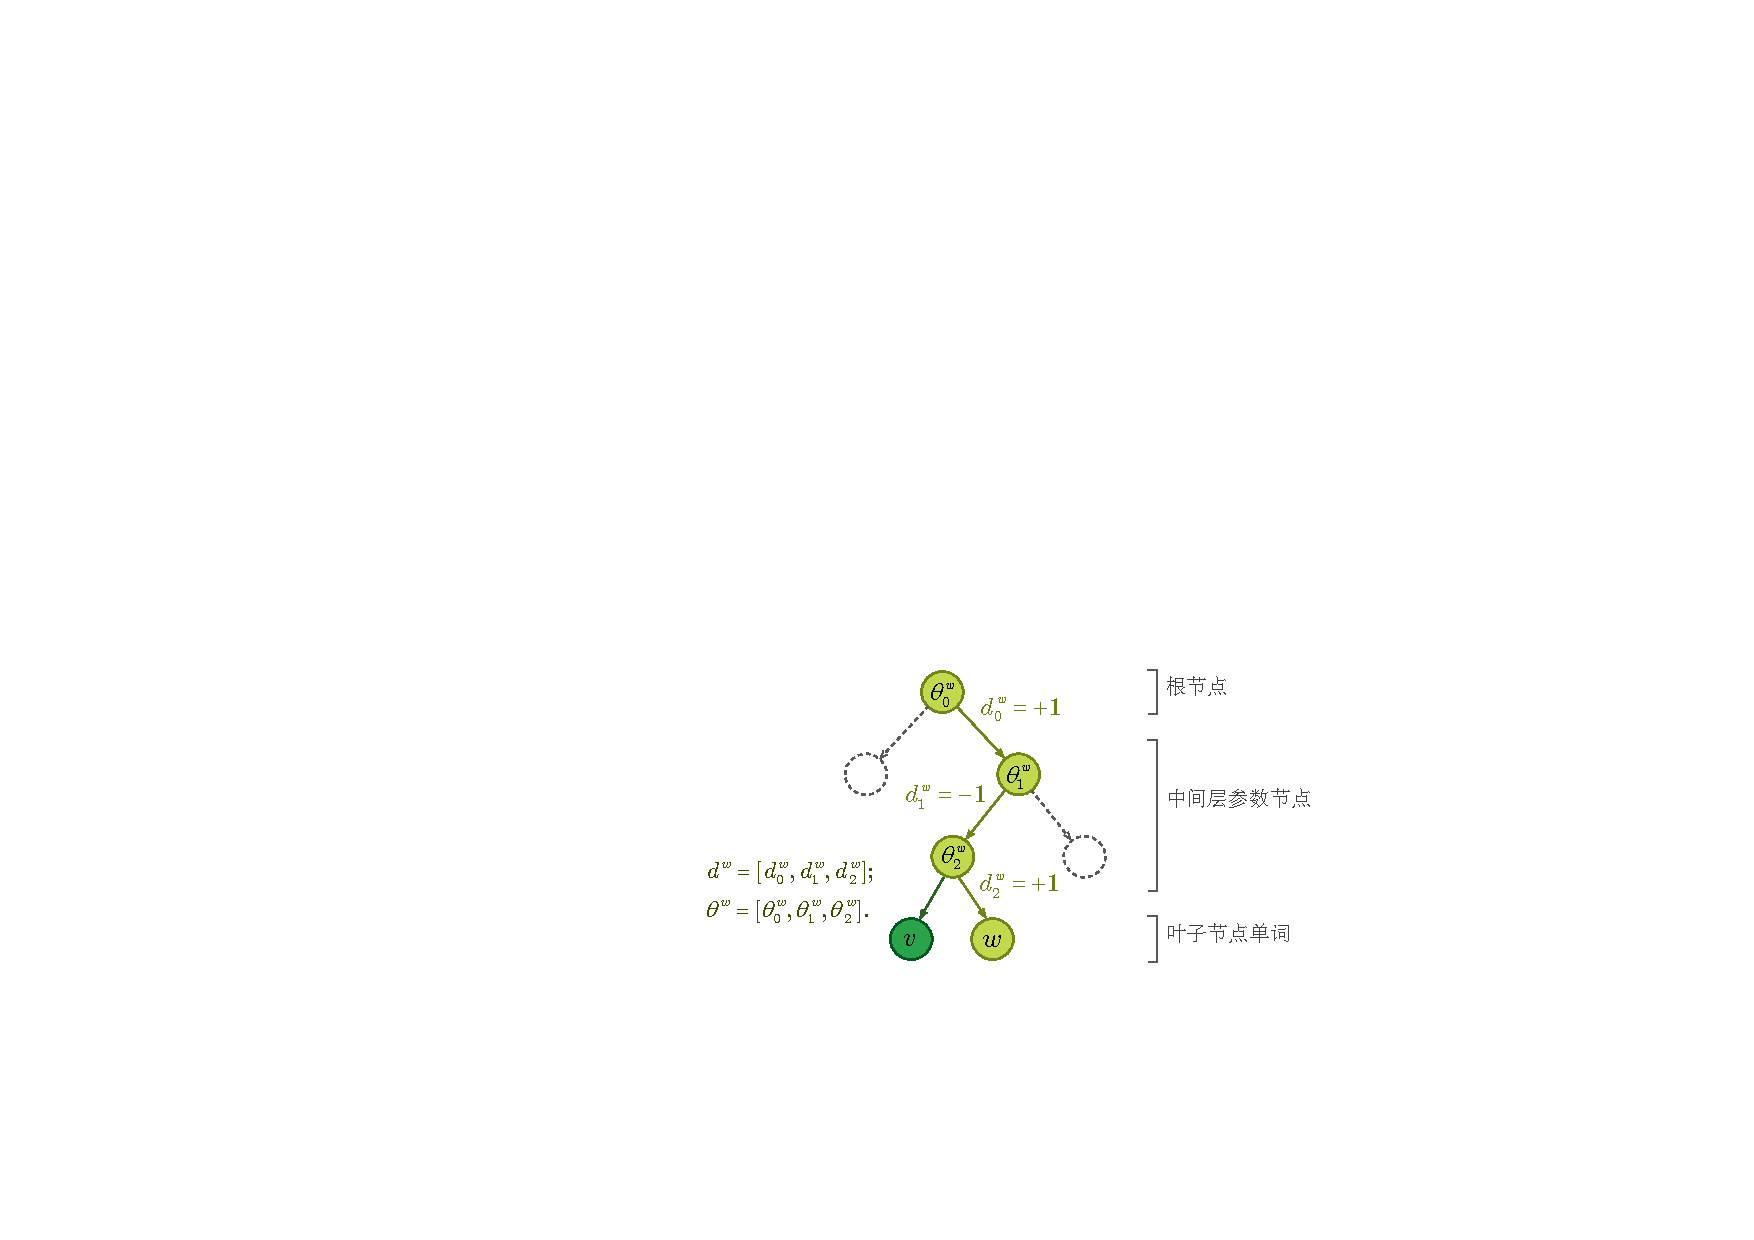
\includegraphics[width=0.93\linewidth]{./figures/thsm.pdf}
\caption{树状层次概率模型}\label{fig:tree_hsm} %
\end{figure}

\section{基于二叉树的代价函数和导数}
接下来给出模型的实际构建过程,如图~\ref{fig:tree_hsm}~所示,模型内部参数向量记为 $\theta_i^w$、 边记为 $d_i^w$,单词在树的叶子节点上。其中, 浅绿色的路径(从根节点到叶子节点~$w$)被定义为参数对 $(d^w,\theta^w)$。这里的 $d^w$ 是一个向量, $\theta^w$ 是一个参数矩阵。例如, 如图中的参数实际结果是 $d^w=[+1,-1,+1]$ , $d^{v}=[+1,-1,-1]$。

在目标词树的每个步骤中,需要对每个非叶节点是左子树还是右子树进行逻辑预测。 所以当给定$ i^{th} $节点和隐藏层的输出向量$h$的时候,可以计算标签 $d^w_i\in \{-1,1\}$的概率为:
 \begin{equation}\label{equ:pp}
 p(d^w_i|\theta_{i}^w,h) =\sigma(\theta_{i}^w h)^{d_i^w}\times(1-\sigma(\theta_{i}^w h))^{1-{d_i^w}},d_i^w \in [0,1]
\end{equation}
其中$ \sigma(z)= 1 /(1 + \exp(-z))$表示 $\sigma$ 函数。根据 $\sigma$ 函数的对称性规则:$\sigma(z)+ \sigma(-z)=1$,可以进一步改造和优化该公式。以下是该公式的具体证明过程如下:
\begin{equation}\label{equ:sig}
\sigma(z)+ \sigma(-z)  =\frac{1}{1 + \exp(-z)}+\frac{1}{1 + \exp(z)}=\frac{1 + \exp(z)}{1 + \exp(z)}=1
\end{equation}
利用$\sigma$ 函数的对称性计算规则将公式~(\ref{equ:pp})~\upcite{minka2003algorithms},缩写成:
 \begin{equation}\label{equ:upper}
p(d^w_i|\theta_{i}^w,h) =\sigma(\theta_{i}^w h)^{d_i^w}, d_i^w \in [-1,+1]
\end{equation}
由于公式~(\ref{equ:upper})~中的其中某一项${d_i^w}$是在指数项上面,所以我们尽管做了这个基于~$\sigma$~函数的变换,我们的计算公式仍然不是最优化的计算形式,仍然还是有空间来提升公式的紧凑性,以保证实际计算过程中的高并行度。更进一步的讲,我们可以将上面的公式缩写成以下形式:
\begin{equation}
p(d^w_i=\pm 1|\theta_{i}^w,h) = \sigma({d_i^w}\theta_{i}^w h)
\end{equation}
我们将指数项移到~$\sigma$~函数计算内部,上述计算公式就是我们所需要用到的计算形态。经过这样的操作之后,我们就完成了单节点概率计算的紧凑表示。针对计算一个单词的概率,我们需要考虑从根节点到该单词叶子节点的所涉及的所有层的概率公式。然而因为在训练的时候,我们实际上预先知道每个单词所对应的路径,所以我们实际上可以同时的计算各个节点的概率值,然后将所有节点相乘起来。这样做的好处将在后续章节进行详细说明。通过以上的操作,虽然在一定程度上增加了计算的复杂度,但是这使得后续在解决计算公式和实际运算流程之间实现一个高效的并行计算成为可能。

因此,对于我们softmax函数计算的单词的条件概率,在这里指的是:单词~$w$~在二叉树上的路径搜寻的概率,即从根到相应叶节点的路径概率$(d^w,\theta^w)$的联合乘积。具体计算公式如下所示:
\begin{equation}\label{equ:pw}
\begin{split}
 \log p(w|h)=&\log\prod_{i=0}^{l^w-1} p(d^w_i|\theta_{i}^w,h) \\
 =& \sum_{i=0}^{l^w -1} \log\sigma(d_i^w \theta_{i}^w h)\\
 =&\log\sigma({d^w}^\top \theta^w h)\\
 =&\zeta(- {d^w}^\top \theta^w h )
 \end{split}
\end{equation}
其中 $\zeta(z)$ 代表的是 softplus 函数: $\zeta(z)= \log (1+\exp(z))$。 该函数的导数是 $\sigma$ 函数~\upcite{DBLP:conf/nips/DugasBBNG00}, 其导数计算公式是:
\begin{equation}\label{equ:zeta}
\begin{split}
\frac{\mathrm{d}\zeta(z)}{\mathrm{d} z}=\frac{\exp(z)}{1+\exp(z)} =\frac{1}{1+\exp(-z)} =\sigma(z)
\end{split}
\end{equation}
如图~\ref{fig:soft}~所示, softplus 函数通常被视为 修正线性单元(Rectified Linear Unit,ReLU)的替代函数,因为他们两个函数除了零点附近分布不一样以外,其他地方分布相同。ReLU函数的计算公式为:$\mathtt{ReLU}(x)=\max(0,x)$。但是softplus函数在零点附近可导,ReLU函数在零点附近不可导。ReLU被使用的更多,因为它能获得近似线性的参数表示,这样能防止模型学习出复杂的表示,缓解模型过拟合问题。
\begin{figure}[!ht]
  \centering
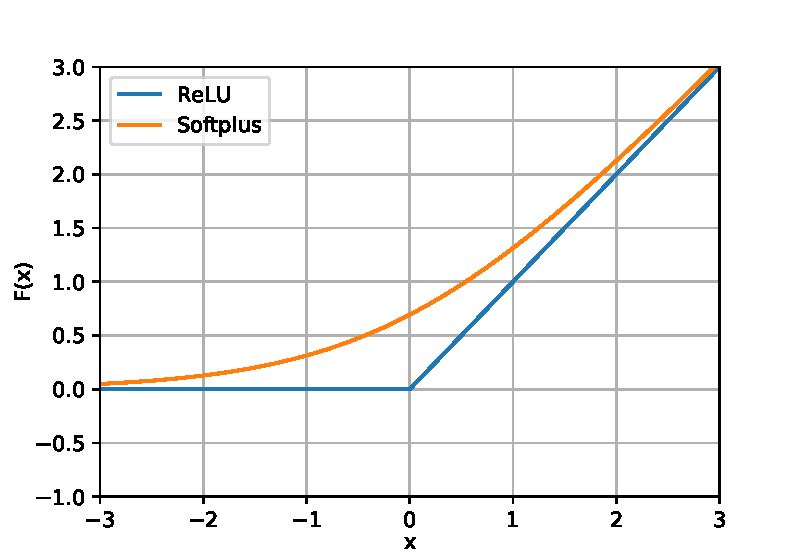
\includegraphics[width=.65\linewidth]{./figures/relus.pdf}
\caption{Softplus和ReLU函数的示意图}\label{fig:soft}
\end{figure}

前面我们已经介绍完模型的单词概率计算公式,接下来我们给出模型相应的损失函数$ \ell(\theta | h,w)$,它是定义在二叉树上面的负对数似然函数(Negative Log-Likelihood,NLL),也可以看作是所有单词概率对数误差的平均值:
\begin{equation}\label{equ:cost}
\begin{split}
   \ell(\theta|h,w) =&-\log\prod_{i=0}^{l^w -1} \sigma(d_i^w \theta_{i}^w h) \\
   =& -\log \sigma({d^w}^\top \theta^w h)\\
    =& \log (1+\exp(- {d^w}^\top \theta^w h )) \\
    =&  \zeta(- {d^w}^\top \theta^w h )
\end{split}
\end{equation}
从此推导公式中,我们可以发现:最小化基于二叉树的负对数似然值,意味着直接最大化softplus损失和下一个单词的分布。

接下来,我们比较一下传统tHSM算法和我们推导获得的p-tHSM算法的异同点。在传统的tHSM算法中,该模型逐层计算每个节点的对数概率。 因此,这个词的整体联合对数概率通过各层线性相加。 从而,tHSM算法的时间复杂度为$\mathcal{O(|H|\log|V|})$,其计算公式为:
\begin{equation}\label{equ:cost2}
\ell(\theta|h,w) =\sum_{i=0}^{l^w-1} \{(1-d'^w_i)\log (\sigma(\theta_{i}^w h))  + {d'^w_i}\log (1-\sigma (\theta_{i}^w h))\}
\end{equation}
其中 $d'^w_i\in \{0,1\}$。我们可以更加形象化的理解这个函数的计算过程:这两个部分对数概率误差从二叉树的叶子底部到根节点,分别对每一层的内部节点的左右子树的联合概率进行合并,其实就是在模仿层次聚类函数从底到顶的合并节点过程。

从公式~(\ref{equ:cost2})所描述的tHSM模型和公式~(\ref{equ:cost})所描述的p-tHSM模型二者计算公式不同,我们可以分析出这两个算法的的主要区别在于:1)tHSM~算法涉及许多微小的矩阵乘法操作,而在~p-tHSM~算法中我们直接将所有参数$(d^w,\theta^w)$ 2D矩阵是以运行时内存消耗为代价的来提高模型单位时间的计算量,我们转而考虑这个向量和相对较大的矩阵的乘法,如图~\ref{fig:tree_hsm}~所示; 2)除了我们的~p-tHSM~模型的损失函数更加紧凑之外,这条路径上所有节点的对数概率而不是逐层计算而是并行的计算,为~p-tHSM~模型提供更好的时间效率。

当我们计算完模型的代价函数后,我们就需要计算模型的参数的导数。接下来,模型的所有参数$\{\theta^w,h\}$针对模型的代价函数的导数是 :
\begin{equation}
\begin{split}
\frac{\partial \ell}{\partial \theta^w}=&(\sigma({d^w}^\top\theta^w h) -1){d^w}^\top h \\
\frac{\partial \ell}{\partial h}=&(\sigma({d^w}^\top \theta^w h) -1){d^w}^\top \theta
\end{split}
\end{equation}


在这个模型中,我们采用二叉树分解的方法,主要是考虑到它一个优点是:它避免了在整个词汇表中计算概率的归一化,因为二叉树中所有的单词的总概率自然等于1。
\begin{equation}
\sum_{w\in \mathcal{V}}{p(w|h)}=\sum_{w \in \mathcal{V}}\sum_{i=0}^{l^w-1}{\sigma(d_i^w\theta_{i}^w h)}=1.
\end{equation}



\section{基于二叉树的推理算法}
接下来我们介绍,在推理阶段层次概率模型所需要解决的主要问题。
\subsection{语句打分任务}
首先,考虑到本章开始提出的第一个问题,即给定序列$ [w_1,\cdots,w_T] $,求该序列出现的概率$   \log p(w_1,\cdots, w_T)$? 直观地说,当给定相应的上下文$ h $时,我们可以通过获取一个特定单词$ w $的概率或对数概率来分解问题:
\begin{equation}
\begin{split}
    p(w|h) =&\sigma({d^w}^\top \theta^w h)\\
   \log p(w|h) =& -\zeta(- {d^{w}}^\top \theta^{w} h )
\end{split}
\end{equation}
其中概率$ p(w|h)$和对数概率$\log p(w | h)$可以直接通过公式~(\ref{equ:pw})~和~(\ref{equ:cost})~逐步计算出来。

因此,我们可以推导出这个序列的概率为:
\begin{equation}
   \log p(w_1,\cdots, w_T)=\sum_{t=1}^T\log p(w_t|h_t) = -\zeta(- {d^{w_t}}^\top \theta^{w_t} h_t )
\end{equation}
显然,这种类型的操作比传统的softmax方法有效得多,因为它只需要$\mathcal{O}(\mathcal {| H | \log| V |})$计算复杂度,而传统的softmax算法却需要$\mathcal{O}(\mathcal {|H||V|})$。

\subsection{单词排序任务}
关于第二种情况(也被称为求解$\arg\max$问题),即当给定一个上下文信息时,在整个词表中搜索最有可能的下一个词(概率最大的单词)。这里的上下文可以指前文、后文或者前后文的窗口。在本实验中,我们所采用的语言模型的情况下,所指代的是前文。

在选择最佳的候选单词之前,词表中所有单词的概率可以被首先计算出,然后将他们按照概率数值大小做排序,获得所有单词的顺序结果。虽然这个过程求解的是全局最优解,但是仍然是相对缓慢的,其计算时间复杂度是$\mathcal{O}(\mathcal{|V|})$,它涉及到遍历整个词表的二叉分层树。如在算法~\ref{alog:global}~中所描述的,为了避免两个小概率的精确度损失问题,我们选择计算每个内部节点的对数概率。


如果我们不采用全局最优搜索算法,而是用局部贪心算法搜索次优结果,那么计算效率能有效提升。具体来说,对于$i$-th层中的节点,当$ p(d^w_i | \theta_{i}^ w,h)\ge 0.5 $时选择左边的子树,相反的情况下选择右子树,如算法~\ref{alog:greed_argmax}~所示。因此,该策略的时间复杂度是$\mathcal{O}(\log\mathcal{|V|})$。

\begin{algorithm}[!ht]
\SetAlgoLined
\KwData{隐藏层输出 $h$;}
 路径列表 $\mathtt{words}$=[] \;
{// 全局概率计算函数}\;
\For{$\theta_w,d_w \in \Gamma(w)$ }{
{$ \log p(w|h)=\zeta(- {d^w}^\top \theta^w h )$}\;
{words.append($\log p(w|h)$)}\;

}
{$\hat w=\arg\max_w{\mathtt{words}}$}\;
\KwResult{ 预测的单词 $w$. }
\caption{全局单词最优算法}\label{alog:global}
\end{algorithm}

\begin{algorithm}[!ht]
\SetAlgoLined
\KwData{隐藏层输出 $h$;}
 路径列表 $\mathtt{route}$=[] \;
 {// 逐层贪心路径搜索}\;
\While{$k \le \log \mathcal{V}$ }{
\eIf{$p(d_{k} |\theta_{k},h) \ge 0.5$ }{
{// 访问左分支}\;
 $k=  k*2$\;
}{
{// 访问右分支}\;
 $k = k*2+1$\;
}
{// 将 $k$ 添加到路径列表}\;
{$\mathtt{route}$.add($k$)}\;
}
{// 通过查找$\Gamma$路径表,找出对应的单词}\;
$w=\Gamma(\mathtt{route})$\;
\KwResult{ 预测的单词 $w$. }
\caption{逐层贪心搜索算法\label{alog:greed_argmax}}
\end{algorithm}



\section{基于二叉树的聚类算法}
词汇表中每个单词的极性编码$(d^w,\theta^w)$与二叉树的结构密切相关,因此对于提出的p-tHSM算法,我们采用了多种树聚类算法来初始化单词在二叉树上的分布,以提高模型的精确性和稳定性。总的来说,这些聚类算法为每个单词生成二进制前缀字符串,表示在树中单词的路径位置,并将用于初始化p-tHSM模型。


1)一元单词聚类算法。它根据文本中单词的词频对单词进行排序,并将词频当作权重从底端到顶端进行合并,该算法也称为霍夫曼编码(Huffman Encoding)~\upcite{DBLP:conf/nips/MikolovSCCD13},算图~\ref{code:huffman}~展示了构造霍夫曼树的过程\upcite{牛雪婷2009Huffman}。如图~\ref{fig:zipf}~所示,我们算法中用到输入信息~$\texttt{freq}$~指的是单词的词频分布,XY基坐标都是对数坐标。


\begin{figure}[!ht]
  \centering
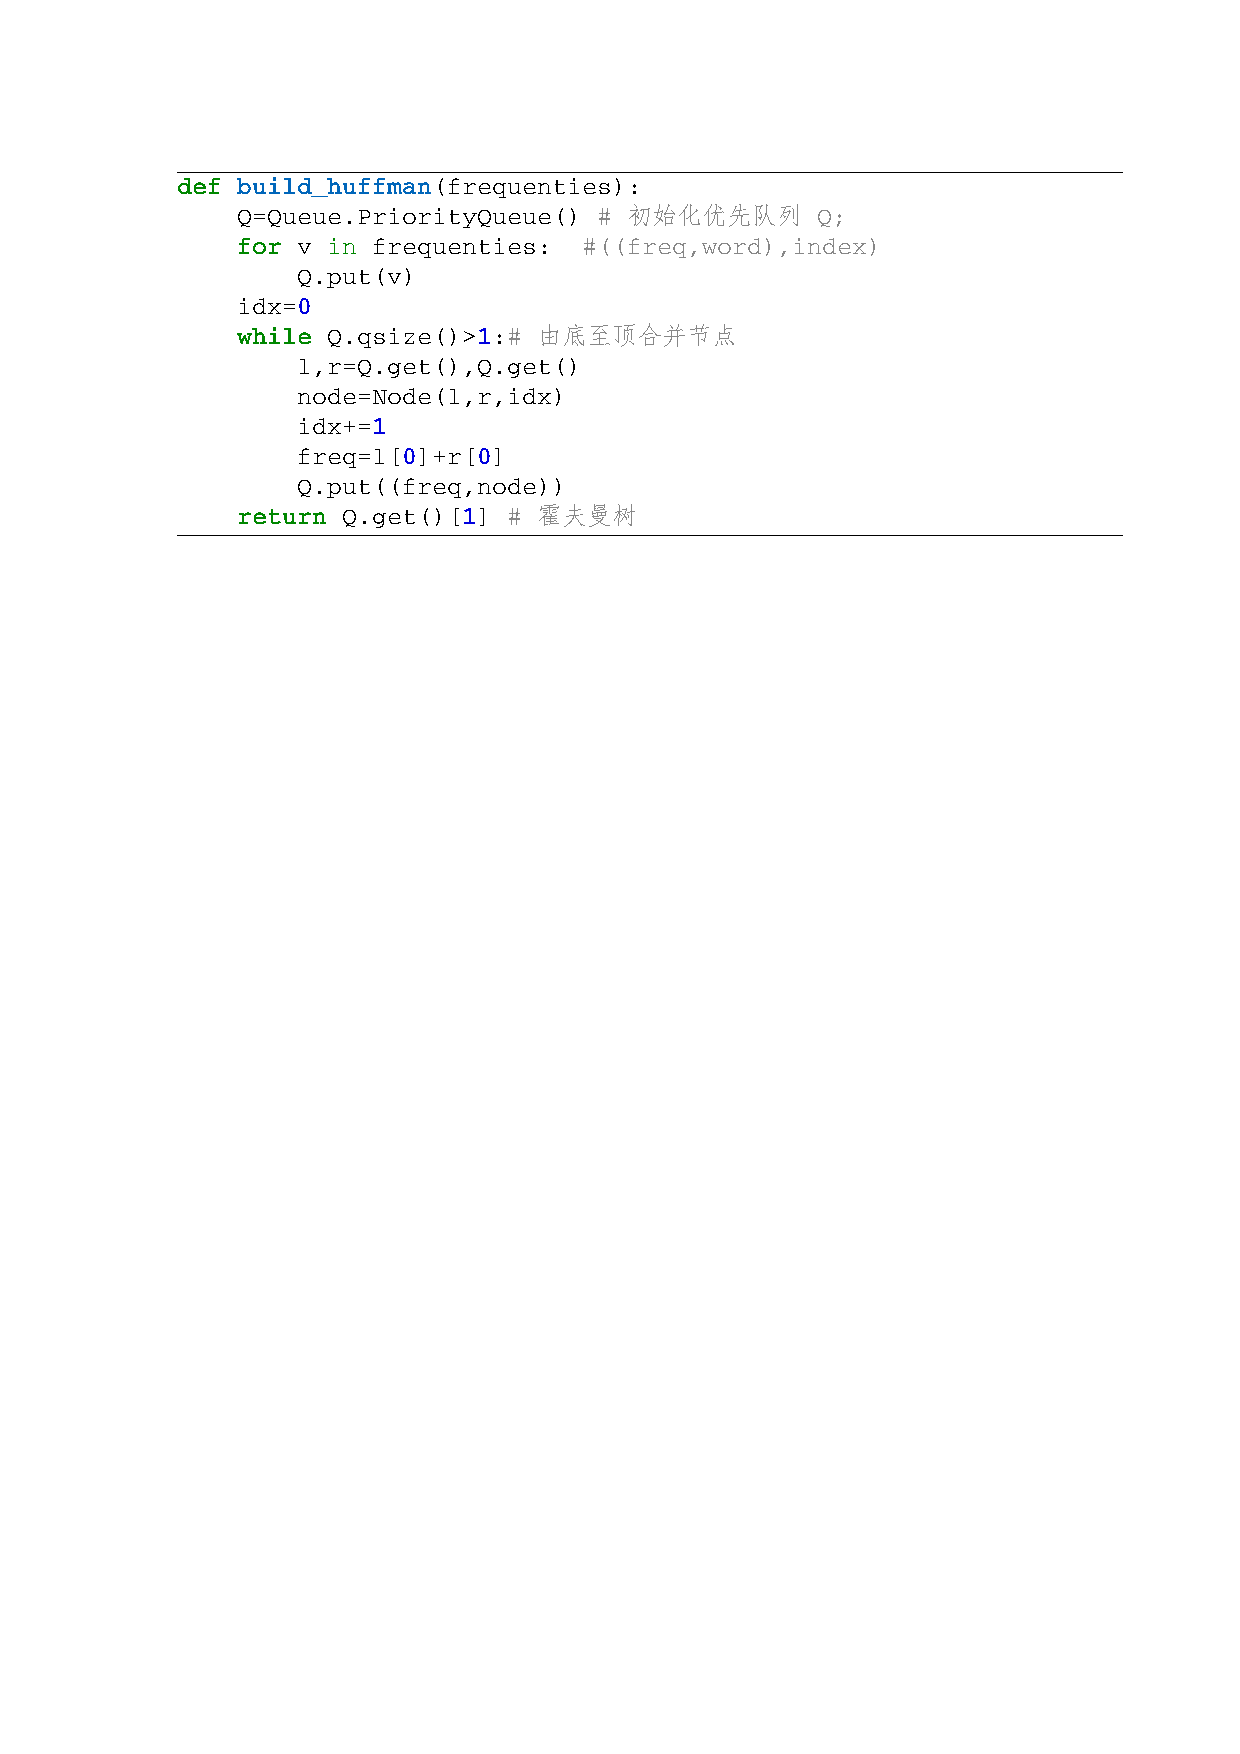
\includegraphics[width=1\linewidth]{./figures/huffman.pdf}
\caption{基于单词频率的霍夫曼建树策略}\label{code:huffman}
\end{figure}

\begin{figure}[!ht]
  \centering
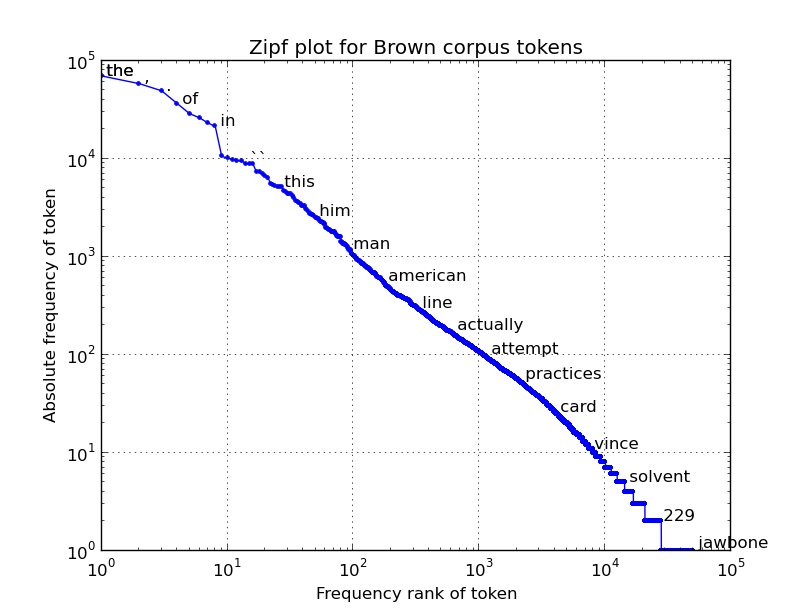
\includegraphics[width=0.85\linewidth]{./figures/zipf.pdf}
\caption{单词词频对数线性分布示意图}\label{fig:zipf}
\end{figure}

当我们构造完霍夫曼二叉树后,我们需要遍历这棵树来获取所有单词的极性编码。1) 首先我们计算待压缩数据中所有的字符及其出现次数,根据次数的不同对每个单词分配不同的权值(一般用出现频率/总字符数); 2) 其次对所有单词按其权值构造一颗霍夫曼树; 3) 对这棵树所有子树的左支用~$-1$~编码,右支用~$+1$~编码。每个位于叶子节点的字符的编码为从根节点到该叶子节点路径上的~$-1,+1$~编码值,这个在树上重新得到的编码称为霍夫曼编码。具体遍历过程可以参考图~\ref{code:preorder},算法的输出单词路径查找表 $\Gamma$就是我们需要提前准备的单词的极性编码。


\begin{figure}[!ht]
  \centering
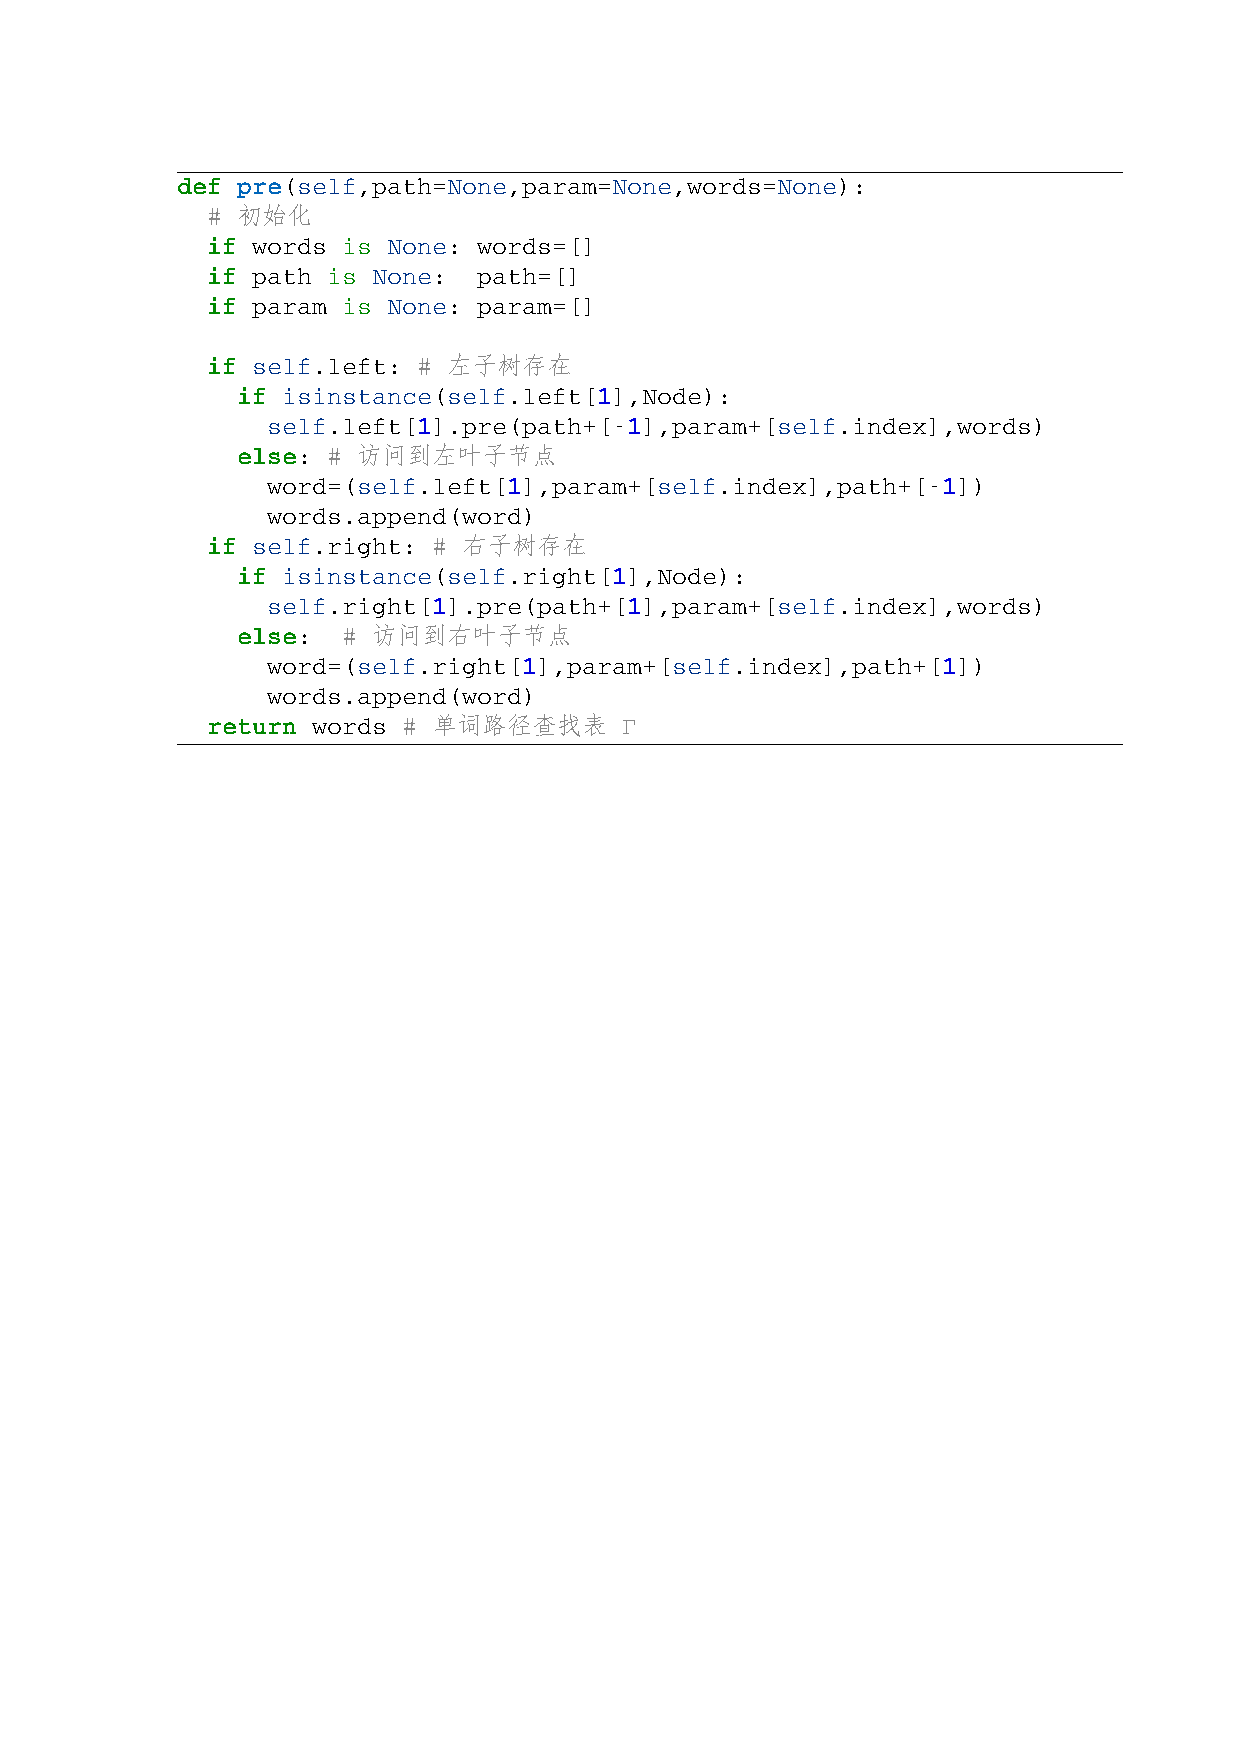
\includegraphics[width=1\linewidth]{./figures/preorder.pdf}
\caption{前序遍历函数生成单词路径查找表}\label{code:preorder}
\end{figure}

\begin{figure}[!h]
  \centering
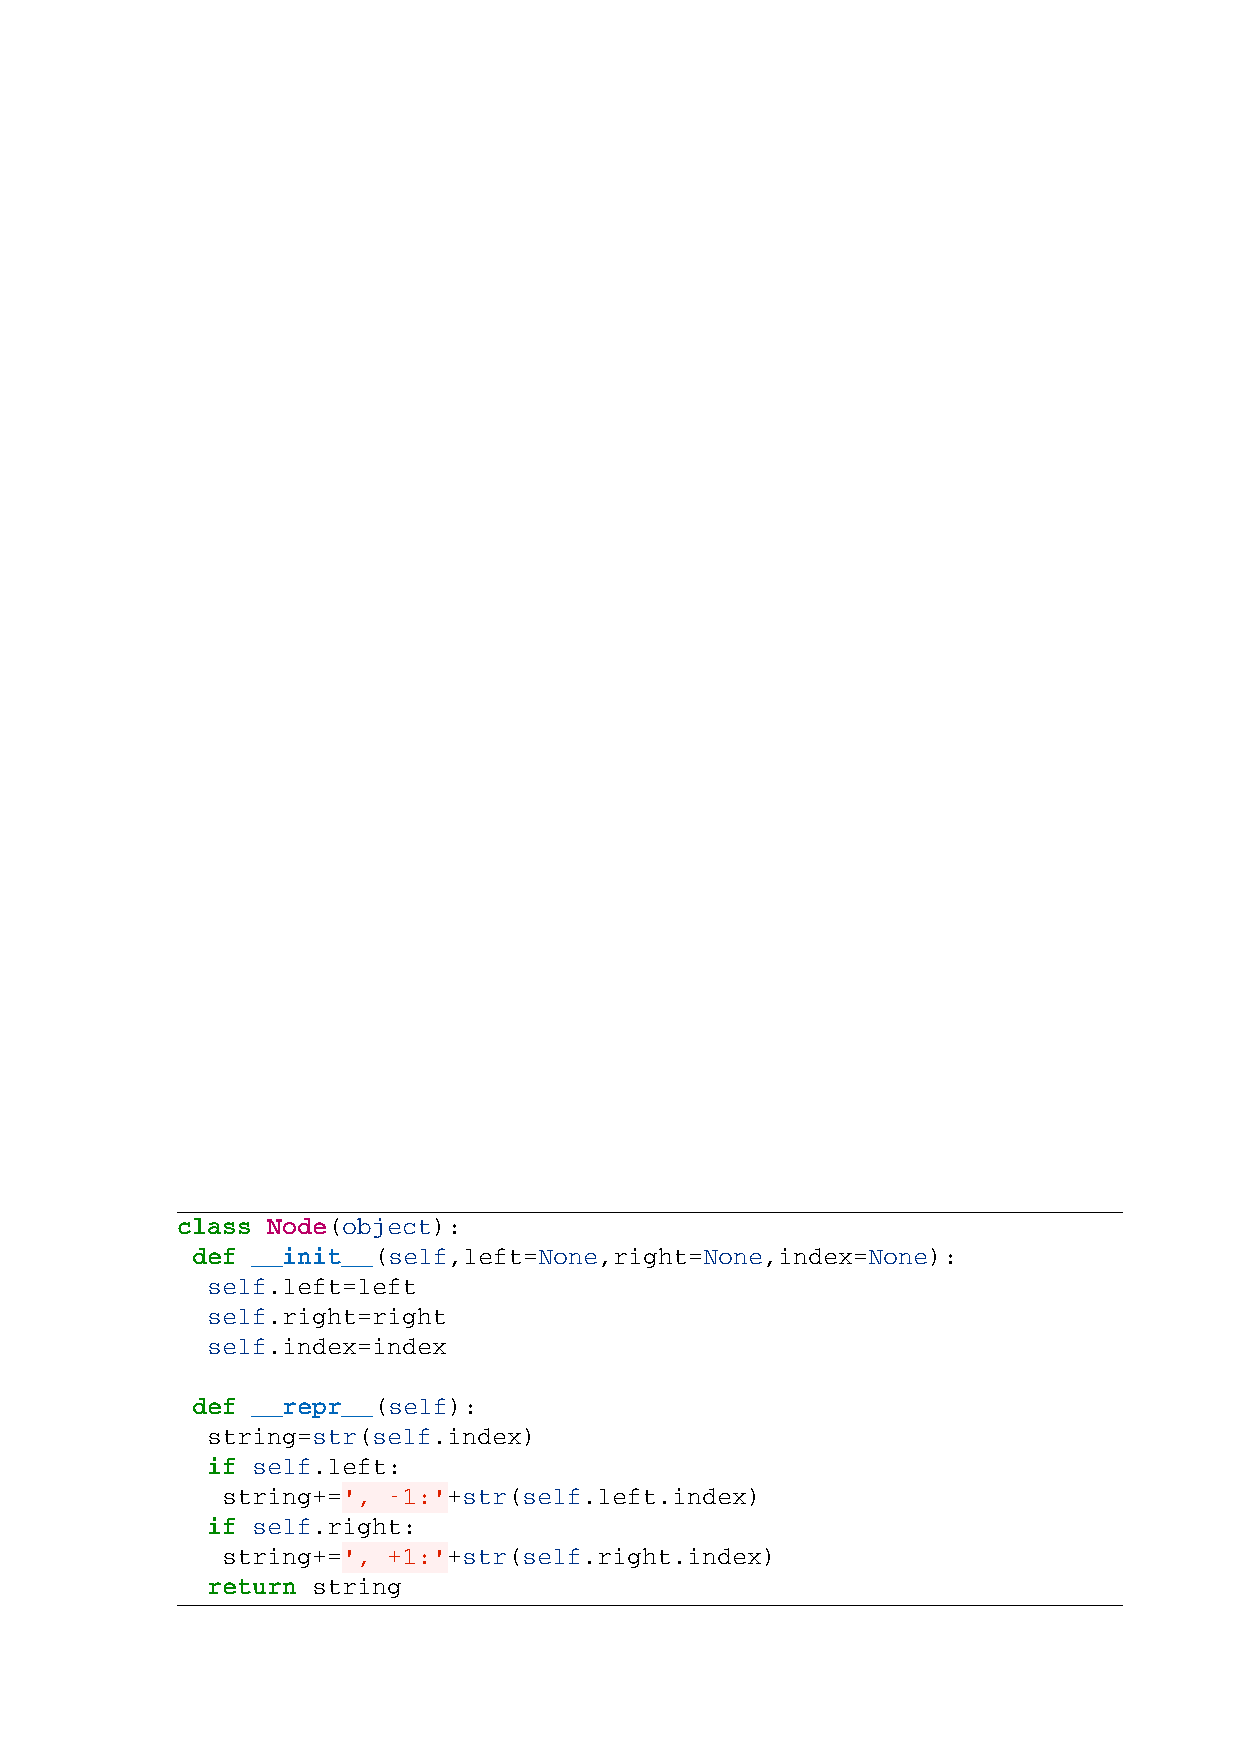
\includegraphics[width=1\linewidth]{./figures/node.pdf}
\caption{基于邻接表的二叉树节点数据组织结构}\label{fig:node}
\end{figure}

上述算法所涉及的模型的各层的节点的实际数据结构如上所示,我们采用邻接表的方式实现。其对应的二叉树的数据结构采用基于数组的方式管理和访问。如图~\ref{fig:node}~所示,每个节点(Node)包含信息为:左子树,右子树和节点编号。同时我们还定义了节点的打印字符串函数(即``\_\_repr\_\_''),方便我们检查数据结构是否正确实现。



2)二元聚类算法\footnote{https://github.com/percyliang/brown-cluster}。它也是一个由底至顶的层次聚类算法,使用Bi-gram上下文信息来确定单词的分布相似性,将相似的单词放置在二叉树的附近位置~\upcite{DBLP:journals/coling/BrownPdLM92,liang2005semi}。算法主要的计算代价就是在于初始化的时候,算法需要计算两两单词之间的距离,对于大词表来说,不断统计~Bi-gram~概率和不断计算两两单词距离是非常费时的。在将簇大小指定为1之后,它从底部到顶部合并具有一个节点的单词,生成的单词路径正是二叉树结构的分布.%样例如下图~\ref{fig:brown}~所示。


3)语义信息聚类算法\footnote{https://code.google.com/archive/p/word2vec/}。这种聚类算法与上面的算法非常相似,其差异点就是:该算法使用单词间的距离尺度是语义向量的余弦相似度(Cosine Distance)。我们需要先调用~Word2vec~或者~Fasttext\footnote{https://github.com/facebookresearch/fastText}~生成所有单词的词向量,然后再初始化两两单词间的距离矩阵。我们需要看到这里的问题是语言模型的其中一个任务也是生成词向量,所以这个操作可以不断自身迭代来提升最后的模型的效果~\upcite{DBLP:books/sp/mining12}。


\section{本章小结}
本章首先定义了极性编码的概念,同时给出了模型所涉及的参数的详细含义。接下来逐步推导模型的单个节点的概率公式,单个词的概率公式和模型的代价函数。另一方面,我们将提出的p-tHSM算法和传统的线性tHSM算法进行的比较,通过对比两者计算的差异性证明我们提出的算法具有更高的计算吞吐量,速度更快。
因为基于二叉树的概率计算方案和传统的softmax计算方案不同,不能直接输出单个词的概率或者计算最佳的候选单词,我们进一步还讨论了模型在测试的时候所需的推理算法,所以我们分别针对排序和打分两个任务提出相应的策略。
最后,由于单词在二叉树上的分布需要初始化,我们概述了传统的霍夫曼聚类算法、布朗聚类算法和语义向量聚类算法。

